\skriptsection{Winkelmodulation (FM/PM)}{68}
Obwohl Winkel- und Frequenzmodulation - im Vergleich zu AM - komplexer ist und mehr Bandbreite
benötigt hat es einen erheblichen Vorteil, welcher die vorhin genannten Nachteile kompensiert.
Nämlich ist die \textbf{Störanfälligkeit} und das \textbf{Rauschen} kleiner als bei AM. \\
\\
Die Grundlage bietet der sinusförmige Träger, wessen Phase oder Frequenz je nach Amplitude des 
Nachrichtensignals moduliert wird.

$$\boxed{ x_c(t) = A \cos(w_c t + \phi(t)) = A \cos(\theta(t)) }$$

\begin{center}
\renewcommand{\arraystretch}{2}
\begin{tabular}{|p{8cm}|p{8cm}|}
	\hline
	\textbf{PM} &	\textbf{FM}\\
	\hline
	$\phi(t) = k_p m(t)$ &
	$ \frac{d \phi(t)}{dt} = k_f m(t) \Rightarrow \phi(t) = k_f \int\limits_{t_0}^{t} m(\lambda)
	d\lambda + \phi(t_0)$\\
	$x_{PM}(t) = A_c \cos[w_c t + k_p m(t)]$ &
	$x_{FM}(t) = A \cos[w_c t + k_f \int\limits_{- \infty}^{t} m(\lambda)
	d\lambda]$\\
	\hline
	$k_p=$ Phasenhubkonstante $[rad]$ & $k_f=$ Frequenzhubkonstante
	$[\frac{rad}{s}]$\\
	\hline
\end{tabular} 
\renewcommand{\arraystretch}{1}
\end{center}


\subsection{Momentanfrequenz, Frequenzabweichung}
\begin{multicols}{2}
	\begin{center}
		$ w_i = \frac{d \theta(t)}{dt} = w_c + \frac{d \phi(t)}{dt} $\\
		$ \Delta \omega = \left| \omega_i - \omega_c \right|_{max} $\\
		$ \Delta f_{FM} =  m_{pk} \cdot \frac{k_f}{2\pi}$\\
		$ \Delta f_{PM} = m_{pk} \cdot \frac{k_p \omega_m}{2\pi} =  m_{pk} \cdot
		k_p f_m$
	\end{center}
\columnbreak

	$\omega_i$ Momentanfrequenz, $[\omega_i] = \frac{rad}{s}$ \\
	$\omega_c$ Trägerfrequenz, $[\omega_c] = \frac{rad}{s}$ \\
	$\Delta \omega$ maximale Frequenzabweichung, $[\Delta \omega] = \frac{rad}{s}$ \\
	$\theta(t)$ momentane Phasenabweichung, $[\theta(t)] = \frac{rad}{s}$ \\
	$m_{pk}$ Peak des Nachrichtensignals
\end{multicols}


\skriptsubsection{Klein- und Grosshub}{70-4.5}
Abhängig von der maximalen Phasenabeweichung sind zwei verschiedene Arten von Winkelmodulationnen zu
unterscheiden. \\

\begin{tabular}{llll}
\textbf{Kleinhub - NB (Narrowband)} 
	& $|\phi(t)|_{max} < 0.2$ 
	& $\Leftrightarrow \quad \beta < 0.2$
	& $\Leftrightarrow \quad D < 0.2$ \\

\textbf{Grosshub - WB (Wideband)}
 & $|\phi(t)|_{max} \gg 1$
 & $\Leftrightarrow \quad \beta \gg 1$
 & $\Leftrightarrow \quad D \gg 1$ \\

\end{tabular}
 


\skriptsubsection{Einton (Sinusförmige)-Modulation (Sinusoidal
Modulation)}{71-4.6}

\subsubsection{Modulationsindex (Modulation Index)}
\begin{minipage}[t][0.7cm][c]{10cm}

$ m(t) = \begin{cases}
          	a_m \sin(\omega_m t)  & \textbf{PM}\\
          	a_m \cos(\omega_m t)  & \textbf{FM}
          \end{cases}  
\qquad
\beta = \dfrac{\Delta \omega}{\omega_m} =
\begin{cases}
	k_p a_m & \textbf{PM}  \\
	\frac{k_f a_m}{\omega m} & \textbf{FM}
\end{cases} 
$
\end{minipage}
\begin{minipage}[t][0.7cm][c]{8cm}
	$\beta$ Modulationsindex (max. Phasenabw.), $[\beta] = rad$ \\
	$a_m$ Amplitude des Nachrichtensignals, $[a_m] = 1$ %\\
	%$k_f$ Frequenzabweichungskonstante, $[k_f] = 1$ \\
	%$k_f$ Phasenabweichungskonstante, $[k_p] = 1$
\end{minipage}

\subsubsection{Spektrum}
$$x_c(t) = A \cos(\omega_c t + \beta \sin(\omega_m t)) \quad \Rightarrow \quad 
x_c(t) = A \sum\limits_{n=-\infty}^{\infty} J_n(\beta) \cos((\omega_c + n \omega_m)t)$$
%%\paragraph{Bessel Funktion}
\textbf{$J_n(\beta)$} ist die \textbf{Bessel Funktion erster Art $n$-ter Ordnung} (Schaum
S. 323f). Das Spektrum besteht aus dem Trägersignal plus einer unendlichen Anzahl Spektrallinien,
wobei $J_n(\beta)$ sehr klein ist für grosse $n$. \\
Für ($\beta \ll 1$, Kleinhub) sind nur $J_0$, $J_1$ und $ J_{-1}$ relevant. Bei ($\beta \gg 1$,
Grosshub) existieren jedoch einige signifikante Seitenbänder.
%%TODO bessel function

\subsubsection{Bandbreite}
Mit der Bedingung $J_n(\beta) \approx 0, \,\forall (n > \beta + 1)$ kann die Bandbreite approximativ
berechnet werden. 98\% der durschnittlichen Signalleistung sind in diesem
Frequenzspektrum angesiedelt. 

\begin{center}
Carson's bandwidth rule: $ W_B \approx 2(\beta + 1) \omega_m = 
	\begin{cases}
  		2 \omega_m (k_p a_m + 1) & \textbf{PM},\, W_B \sim \omega_m \\
  		2(k_f a_m + \omega_m) & \textbf{FM},\, W_B \nsim \omega_m \end{cases} \qquad
  		\qquad \qquad \beta < 0.2 \text{ (NB)}: \quad W_{B} \approx 2 \omega_m
$
\end{center}
F\"ur Frequenzen in Zeitbereich ($Hz$) kann $\omega_m$ mit $f_m$ und
$\omega_{\Delta}$ mit $f_{\Delta}$ ersetzt werden.\\
\subsubsection{Leistung \formelbuch{78-4.6}}
$$P = \frac12 A_C^2$$



\subsection{Willkürliche-Modulation (Arbitrary Modulation) \formelbuch{72-4.7B}}
Anstelle von $\beta$ verwenden wir für willkürliche Nachrichtensignale $D$ für die
Phasenabweichung.\\ 
\begin{minipage}[t][2.7cm][c]{10cm}
	$$ D = \frac{\Delta \omega}{W_M} $$	
$$\text{Carson's bandwidth rule:} \quad W_B \approx 2(D + 1) W_M $$ 
$$ \textbf{NB}(\forall (D \ll 1)): \quad W_{B} = 2 W_M $$ 
$$ \textbf{WB} (\forall (D \gg 1)): W_{PM} = 2 \Delta \omega \text{(prop. $W_M$)};
 \quad W_{FM} = 2 \Delta \omega ~\text{(const.)} $$
\end{minipage} \hspace{0.6cm}
\begin{minipage}[t][2.7cm][c]{8cm} 
	$D$ Modulationsindex = max. Phasenabw., $[D] = rad$ \\
	$W_M$ Bandbreite des Nachrichtensignals \\
	$\Delta \omega$ Frequenzabweichung \\
	$W_B,W_{FM},W_{PM}$ Bandbreite des winkelmodulierten Signals
\end{minipage} \\
Bei Grosshub-FM bleibt die resultierende Bandbreite $W_{FM}$ bei ändernder Nachrichtenbandbreite
$W_M$ gleich. Bei Grosshub-PM ändert sich diese Bandbreite$W_{PM}$ jedoch proportional zur
Nachrichtenbandbreite $W_M$.\\


\subsection{Modulationsarten}
Auch bei der Modulation muss zwischen Klein- und Grosshub FM/PM unterschieden werden.

%pm_nbpm_modulator.png fm_nbfm_modulator.png

\skriptsubsubsection{Kleinhub Modulation}{72-4.8A}
Aus der trigonometrische Gleichung ($\cos(\beta + \alpha) = \cos(\alpha) \cdot \cos(\beta) -
\sin(\alpha) \cdot \sin(\beta)$ mit $\cos(\alpha) \approx 1, \sin(\alpha) \approx \alpha$) ergibt
sich: \\
$$\cos(\beta) - \alpha \cdot \sin(\beta) \quad \Rightarrow \quad \cos(\omega_c t + k_p \cdot m(t))
= \cos(\omega_c t) - k_p \cdot m(t) \sin(\omega_c t)$$

\begin{minipage}[t][3cm][c]{9cm}	
	\begin{center}
  		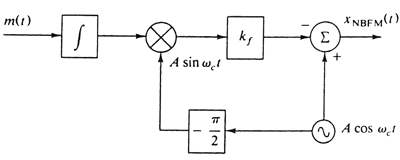
\includegraphics[height=2.8cm]{bilder/fm_nbfm_modulator.png} \\
  		\textbf{Kleinhub-FM Modulator}
	\end{center}
\end{minipage}
\begin{minipage}[t][3cm][c]{9cm} 
	\begin{center}
		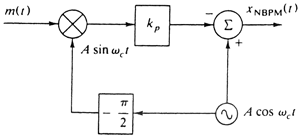
\includegraphics[height=2.8cm]{bilder/fm_nbpm_modulator.png} \\ 
  		\textbf{Kleinhub-PM Modulator}
	\end{center}
\end{minipage}

\skriptsubsubsection{Indirekte Grosshub Modulation}{73-4.8B1}
\begin{minipage}[t][3cm][c]{10cm}	
	Bei dieser Methode wir zuerst ein Kleinhub-Signal erzeugt und dann mittels einem
	\textbf{Frequenzmultiplikator} in ein Grosshub-Signal gewandelt.
	$$ x(t) = A \cos[\omega_c t + \Phi(t)] \quad \Rightarrow \quad y(t) = A \cos[n \omega _c t + n
	\Phi(t)]$$ Frequenzmultiplikation ist realisierbar mit nicht-linearen Bauteilen (Diode, Transistor,
	etc.).
\end{minipage}
\begin{minipage}[t][3cm][c]{8.5cm} 
	\begin{center}
		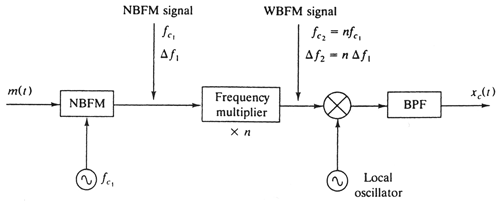
\includegraphics[height=3.4cm]{bilder/fm_nbfm2wbfmConverter.png}
	\end{center}
\end{minipage}

\skriptsubsubsection{Direkte Grosshub Modulation}{74-4.8B2}
Dank der spannungsabhängigen Sperrschichtkapazität von Dioden (Varicap - Kapazitätsdiode,
Dioden-Varaktor, MOS-Varaktor) ist es möglich spannungsabhängige Oszillatoren zu entwickeln. Diese \textbf{VCOs
(Voltage Controlled Oscialltor)} können dann direkt ein Grosshub PM/FM Signal
erzeugen.\\


\subsection{Demodulation}
Die Demodulation von FM benötigt ein System, welches eine Ausgangsspannung proportional zur
momentanen Frequenzabweichung erzeugt, solch ein System nennt man Frequenzdiskriminator. \\
Auch PM kann so einfach demoduliert werden, indem am Ausgang des FM-Demodulators noch ein
Integrator nachgeschalter wird.

\subsubsection{Frequenzdiskriminator}
\begin{minipage}[t][3cm][c]{6cm}	
	\begin{center}
  		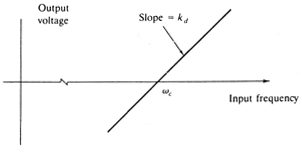
\includegraphics[height=2.8cm]{bilder/fm_pm_frequenzdiskriminatorAmplitudengang.png} \\
  		\textbf{Idealer Frequenzdiskriminator}
	\end{center}
\end{minipage}
\begin{minipage}[t][3cm][c]{6cm} 
	Praktisch wird der Frequenzdiskriminator durch ein Differentiator mit nachgeschaltetem
	Envelope-Detektor realisiert.
\end{minipage}
\begin{minipage}[t][3cm][c]{6cm} 
	\begin{center}
		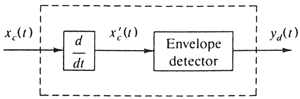
\includegraphics[width=5cm]{bilder/fm_pm_frequenzdiskriminatorRealisierung.png} \\ 
  		%\textbf{}
	\end{center}
\end{minipage}

\subsubsection{PLL - Phase-Locked Loop}
Bei einem PLL handelt es sich um einen phasengekoppelten Regelkreis. Dieser vergleicht die
aktuelle Frequenz eines internen Oszillators (VCO) mit einer Referenzfrequenz. Sollte die
interne Frequenz von der Referenzfrequenz abweichen, wird diese nachgeregelt. \\
Aus der Steuerspannung für den internen Oszillator resultiert genau die Frequenzabweichung und
somit auch das ursprünglich FM-modulierte Nachrichtensignal.\\


\subsection{UKW Radio}
Das UKW Signal besteht primär aus zwei Audiosignalen: Dem Summen- (L+R) und dem Differenzsignal (L-R).
Somit kann bei schlechtem Empfang nur Mono (L+R) und bei gutem Empfang Stereo (L/R) gehört werden. \\
Zur Synchronisation mit dem Demodulator dient der 19kHz Pilot Ton. \\
Mit RDS (Radio Data System) werden Digitale Daten wie z.B. Senderinformationen (Sendername, Uhrzeit,
\ldots) mit einer Datenrate von 1187.5 bit/s übertragen. \\
\begin{minipage}{9cm}
	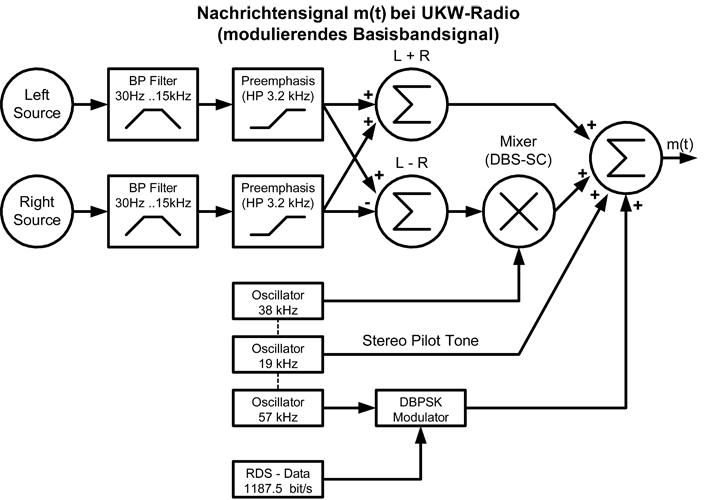
\includegraphics[width=7cm]{bilder/ukw_blockdiagramm.png}
\end{minipage}
\begin{minipage}{9cm} 
	\textbf{Spektrum des UKW Nachrichtensignals} \\ \\
    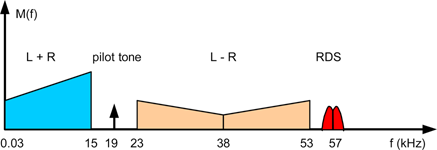
\includegraphics[width=8cm]{bilder/ukw_spektrum.png}
\end{minipage}
